\documentclass[a4paper,14pt,twoside]{extarticle} \usepackage[utf8]{inputenc}
\usepackage[T1]{fontenc}
\usepackage[margin=2.5cm]{geometry}

% Fonte Caladea se existir, senão lmodern
\IfFileExists{caladea.sty}{
  \usepackage{caladea}
}{
  \usepackage{lmodern} }
\usepackage{ragged2e}
\usepackage{graphicx}
\usepackage[portuguese]{babel}
\usepackage{wrapfig}
\usepackage{hyperref}
\usepackage{fancyhdr}
\usepackage{xcolor}
\usepackage{rotating}
\usepackage{titlesec}
\usepackage{epigraph}
\usepackage{dirtytalk}
\usepackage{indentfirst} % Indenta o primeiro parágrafo após seções

% Ajuste do recuo de parágrafo
\setlength{\parindent}{1.5em}

% Centralizar títulos
\titleformat{\section}
  {\normalfont\centering\bfseries\Large}{\thesection}{1em}{}

\titleformat{\subsection}
  {\normalfont\centering\bfseries\large}{\thesubsection}{1em}{}

\titleformat{\subsubsection}
  {\normalfont\centering\bfseries}{\thesubsubsection}{1em}{}

% -------------- Símbolos de Versículo e Resposta --------------
% Definição do símbolo (a “barrinha” inclinada)
\makeatletter
\newcommand{\vers@resp@sym}{%
  \raisebox{0.2ex}{\rotatebox[origin=c]{-20}{$\m@th\rceil$}}%
}
% macro interna que sobrepõe a barrinha e a letra V ou R
\newcommand{\vers@resp}[2]{%
  {\ooalign{%
     \hidewidth\kern#1\vers@resp@sym\hidewidth\cr
     #2\cr
  }}%
}
% comandos públicos \versicle e \response
\DeclareRobustCommand{\versicle}{\vers@resp{-0.1em}{\textbf{V}}}
  \DeclareRobustCommand{\response}{\vers@resp{0pt}{\textbf{R}}}
\makeatother
% ^------------- Símbolos de Versículo e Resposta -------------^

% Rodapé com imagem e página
% Ajuste para cabeçalho do fancyhdr
\setlength{\headheight}{18pt} % Ajuste recomendado pelo warning do fancyhdr
\pagestyle{fancy}
% ---- Cabeçalho ------------
\fancyhf[C]{}
% ----- Rodapé --------------
\fancyfoot[LO,LE]{%
  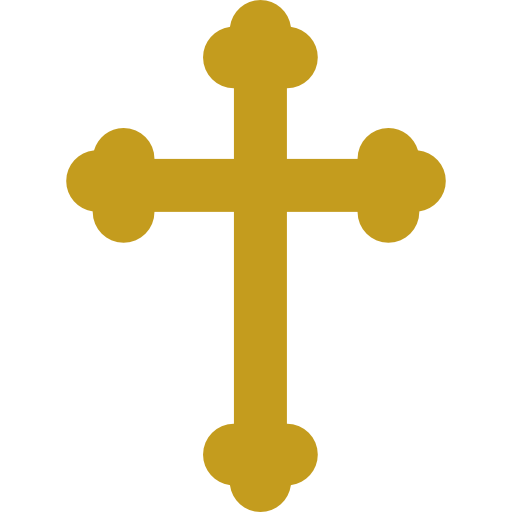
\includegraphics[scale=0.2]{assets/cross.png}\quad
  \textit{Novena a \textbf{Nossa Senhora de Rocio}}
}
\fancyfoot[RO,RE]{\thepage}

\begin{document}


\begin{center}
  {\huge Novena a Nossa Senhora de Rocio}
\end{center}


A palavra “Rocio” vem do Latim “Roscivum”, que significa “orvalho”. E o uso do termo orvalho aplicado a esse título de Nossa Senhora simboliza as bênçãos e as graças recebidas das mãos de Nossa Senhora. Graças estas que brotam constantemente no meio do povo como o orvalho.


{\centering \rule{1.0\textwidth}{0.4pt}}

\tableofcontents
\thispagestyle{empty}


\newpage
\section{História}

\subsection{PADROEIRA DO PARANÁ}

A devoção a Nossa Senhora do Rocio teve início no século XVII, logo após a elevação do pelourinho em Paranaguá, em 1648. Quando, em 1686, os habitantes desta Vila, às margens de sua baía, foram assolados por uma peste, essa gente recorreu aos favores de Maria Mãe de Jesus, invocada neste título, para que os livresse desta terrível lamúria. Desde aí, Nossa Senhora do Rocio vem sendo o socorro das aflições dos devotos cristãos paranaenses. Rocio era o perímetro das Vilas, onde terminava a povoação, o arruamento, e começava a se condensar orvalho matutino. Rocio quer dizer orvalho, em português arcaico. Nossa Senhora do Rocio é Nossa Senhora do Orvalho Matutino, Nossa Senhora do Amanhecer. A imagem da Virgem do Rocio foi encontrada numa pesca milagrosa, nas redes do Pai Berê, no século XVII, na baía de Paranaguá. A primeira igreja foi edificada em 1813 e o Santuário em 1920.

Devido aos muitos milagres e graças alcançadas por intercessão, a devoção se espalhou entre o povo do Paraná e de diversos lugares as multidões faziam romarias ao Santuário da Virgem do Rocio. Assim, em 1977 o Papa Paulo VI declarou para a eternidade Nossa Senhora do Rocio como a Padroeira do Paraná. Está crescendo, a cada dia que passa, a devoção a Virgem e Mãe do Rocio e consequentemente seu Santuário, em Paranaguá, está sendo cada vez mais visitado pelos devotos e turistas.

 
\subsection{MILAGRES ATRIBUIDOS A NOSSA SENHORA DO ROCIO}

Através dos anos, a devoção cresceu até o milagre que deu fim a peste, em 1686, milagre que se repetiu ao longo dos séculos em inúmeras ocasiões em que a Santa do Rocio atendeu aos seus devotos com curas individuais e coletivas, como nos casos da Peste Bubônica, em 1901 e da Gripe espanhola, em 1918.

Há ainda inúmeros registros do socorro da Virgem do Rocio prestado aos marinheiros em violentas tempestades e tragédias no mar, os quais se tornaram seus devotos e a homenagearam com procissões e comoventes romarias pelas ruas da cidade, rumo ao Santuário. É o caso do navio “Raul Soares”, no dia 26 de junho de 1931; do navio “Philadélphia”, em julho de 1931; e do navio “Maria M”, no dia 08 de agosto de 1932.

 
\subsection{O TÍTULO DE PADROEIRA DO PARANÁ}

Além desses, contam-se, muitos outros milagres ocorridos em cidades do Paraná sob sua intercessão, razão pela qual, em 1939, Nossa Senhora do Rocio foi declarada Padroeira do Paraná pelos Bispos do Estado e, finalmente, após anos de esforço civil e eclesiástico, a Santa Sé a declarou, em 1977, Padroeira do Paraná, indicando a Igreja do Rocio em Paranaguá como seu Santuário Estadual.

O título de Rocio, que na linguagem antiga significa “orvalho”, simboliza as constantes e ininterruptas bênçãos e favores que o povo paranaense recebe continuamente da Virgem Mãe, mediadora de todas as graças concedidas a seus amados filhos, os quais, por gerações e gerações, veneram sua Santa Padroeira as margens da baía de Paranaguá sob o titulo de Senhora do Rocio.

\subsection{CONGREGAÇÃO REDENTORISTA: BREVE HISTÓRIA DOS REDENTORISTAS}

Santo Afonso Maria de Ligório fundou em 1732 no sul da Itália a Congregação do Santíssimo Redentor, popularmente chamada Congregação dos Redentoristas.
Os Redentoristas se esforçam por continuar o exemplo de Jesus Cristo Redentor pregando o Evangelho aos pobres (cf. Lc 4,14-21).

A Congregação teve início como uma resposta às necessidades espirituais dos abandonados, do povo pobre que vivia na zona rural, nas montanhas fora da cidade de Nápoles.

A princípio, apenas uns poucos homens seguiram a inspiração de Santo Afonso. Mas enquanto ainda vivia o Fundador, a Congregação expandiu-se para fora do Reino de Nápoles, primeiramente para a Itália central e depois para a Polônia.

Durante as primeiras décadas do séc. XIX foram fundadas comunidades redentoristas no Império austro-húngaro, na Alemanha, na Bélgica e na Holanda.

Em 1832, no centenário da fundação da Congregação, seis missionários redentoristas (três sacerdotes e três irmãos) partiram para os Estados Unidos e começaram a primeira obra missionária fora da Europa. Seguiram-se fundações na América Latina, na Austrália e depois na África e na Ásia.

 
\subsection{MISSIONÁRIOS REDENTORISTAS}

Os Missionários Redentoristas, padres e irmãos, estão espalhados pelo mundo inteiro, presente em mais de 80 países. Em 1894 chegaram os primeiros Redentoristas no Brasil. Atualmente somos aproximadamente 600 missionários aqui no país, distribuídos em nove unidades, que são cinco (5) Províncias: Rio de Janeiro, São Paulo, Porto Alegre, Goiás e Campo Grande, e quatro (4) Vice Províncias: Recife, Fortaleza, Manaus e Bahia.

Nós da Província de Campo Grande, estamos nos Estados do Paraná e Mato Grosso do Sul. Cuidamos de paróquias, santuários e meios de comunicação social. A Congregação do Santíssimo Redentor é um Instituto clerical de vida apostólica e votos simples, com a finalidade de: “continuar o exemplo de Jesus Cristo Salvador, pregando aos pobres a Palavra de Deus, como disse de si mesmo: Enviou-me para evangelizar os pobres” (Const. 1). “Os membros da Congregação tem como incumbência o anuncio explicito do Evangelho” (Const. 5). “Esse anuncio visa especialmente a Copiosa Redenção, isto é, o amor de Deus Pai “que nos amou primeiro e nos enviou seu Filho, como propiciarão pelos nossos pecados” (1Jo 4, 10) e que pelo Espírito Santo vivifica a todos os que n’Ele creem” (Const. 6).

Desde o começo eles corresponderam à vocação com exercícios espirituais, missões e Instrução religiosa. A Congregação foi fundada em Scala no dia 09 de novembro de 1732, na Itália, por Santo Afonso Maria de Ligório. No começo foi uma simples Congregação de padres seculares sem votos, mas em 1740 para assegurar uma estabilidade maior, eles fizeram o voto de perseverança. Depois da morte de Falcoia em 1743, a Congregação, ou o Capítulo, escolheu Santo Afonso como superior maior com o título de Reitor mor e, ao mesmo tempo, eles adotaram os três votos religiosos. Depois da profissão religiosa de São Clemente Maria de Hofbauer e do Padre Thaddeus Hübl, em 1785, a Congregação se estendeu às regiões do Norte da Europa. Em 1787 uma comunidade foi fundada em Varsóvia. Depois da morte de São Clemente, em 1820, e sob a direção do Venerável Padre José Passerat, Vigário Geral fora da Itália, a Congregação conheceu uma expansão considerável até chegar aos Estados Unidos.

\newpage


\section{Novena a Nossa Senhora de Rocio}
\subsection*{Oração de Todos os Dias}
Em nome do Pai, do Filho e Do Espírito Santo.

Nossa Senhora do Rocio, agradecemos a vossa intercessão maternal. Em Jesus, louvamos o nosso Deus misericordioso por todas as graças e bênçãos recebidas. Ó Mãe, olhai para todas as nossas necessidades. Por vossa intercessão, que os céus se abram e sobre nós orvalhos de bênçãos sejam derramados. Pedimos por nossas famílias, pelos doentes e excluídos. Mãe, que a nossa Igreja seja cada vez mais fortalecida e sinal de serviço. Que o Reino da paz, justiça e do amor prevaleçam. Que a misericórdia entre nós seja abundante.

Lembrai-vos, Virgem Santíssima, que jamais se ouviu dizer, tendo alguém necessitado recorrido a vós, implorado o vosso auxílio e reclamado o vosso socorro, fosse por vós desamparado. Com igual confiança, Virgem e Mãe do Rocio, animado peço pela minha família, pela minha comunidade, pelos doentes e aflitos e por mim mesmo. Ó Mãe amável, rogai por nós, para que sejamos dignos das promessas de Cristo.

\vspace{1cm}

\versicle. Rogai por nós, Nossa Senhora do Rocio.

\response. Para que sejamos dignos das promessas de Cristo.

\vfill

\begin{center}
\subsection*{Fontes:}
Adaptado de: 
 \underline{\href{https://www.vaticannews.va/pt/santo-do-dia/11/11/s--martinho--bispo-de-tours-.html}{Vatican News}}, \underline{\href{https://www.praymorenovenas.com/st-martin-of-tours-novena}{Pray More Novenas}} e \underline{\href{https://santo.cancaonova.com/santo/sao-martinho-de-tours-o-dono-do-manto-que-cobriu-jesus/}{Canção Nova}}.
\end{center}


\end{document}
